\section{实验结果}
\subsection{网络拓扑与数据流向}
如图\ref{HTTP}所示,用户通过Web客户端应用程序(即浏览器)向
Web服务器发出请求,请求通过HTTP协议送到
Web服务器;Web服务器根据Web客户端的请求将
保存在Web服务器中的某个页面通过HTTP协议返
回给Web客户端;浏览器接收到页面后对其进行解
释,最终将图、文、声并茂的画面呈现给用户。
\begin{figure}[!htbp]
    \centering
    \includegraphics[width=\textwidth]{figures/HTTP.pdf}
    \caption{网络拓扑和数据流向}\label{HTTP}
\end{figure}
\subsection{WEB页面构成}
\begin{figure}[!htbp]
    \centering
    \includegraphics[width=\textwidth]{figures/HTML.pdf}
    \caption{\url{google.co.jp}的页面构成}\label{HTML}
\end{figure}
如图\ref{HTML}所示,我将\url{google.co.jp}的页面按照组件进行拆分,红、黄、绿、蓝分别代表组件树中的第一、二、三、四层。
在HTML文件中,第一层是<html>元素,第二层是<head>和<body>元素。其中,<head>中存储着页面的元信息等内容,如字符编码,显示风格,页面的标题等;
<body>中存储着图\ref{HTML}中所划分的组件树,除此之外,还有用于描述页面样式的<style> 元素和交互逻辑的<script> 元素。

<div>元素是流式内容的通用容器。它对内容或布局没有影响;
<img>元素将一张图像嵌入文档;
<center>元素是一个块级元素,它在其包含元素中将其块级或行级内容水平居中显示;
<a>元素(或称锚元素)可以通过它的 href 属性创建通向其他网页、文件、电子邮件地址、同一页面内的位置或任何其他 URL 的超链接。
\subsection{HTTP协议}
\subsubsection{GET方法}
图\ref{GET1},\ref{GET2}为\url{google.co.jp}发出的一个GET方式的请求和对应响应的报文内容。

在General菜单中,Request URL字段表明该请求所需资源的URL为\url{https://www.google.co.jp/favicon.ico};
Request Method字段表明该请求的方法为GET;
Status Code字段表明请求成功,状态码为200。

在Response Headers菜单中,
Cache-Control字段表明该客户端和代理服务器都可以缓存该条数据,缓存时间为619200秒;
Content-Encoding,Content-Length和Content-Type字段分别说明了该数据的编码方式、长度以及类型。

在Request Headers菜单中, 
Referer字段表明该请求从\url{https://www.google.co.jp/}发送;其他字段说明了客户端的各种属性,例如颜色风格为暗色、使用Google Chrome游览器、
CPU架构为x86等等。


\begin{figure}[!htbp]
    \centering
    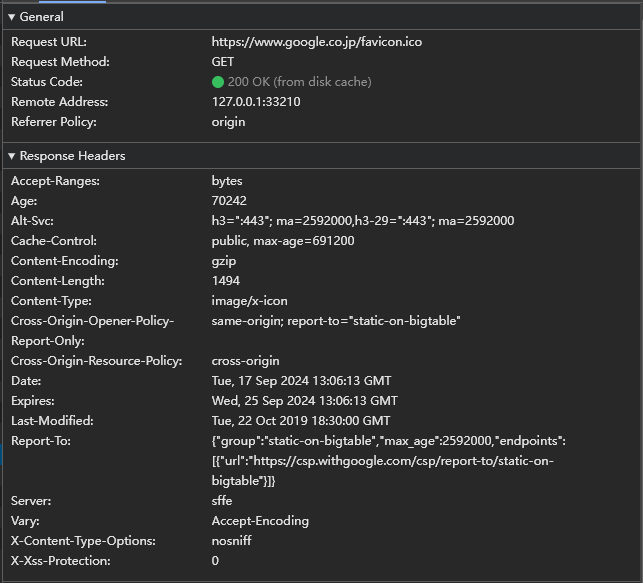
\includegraphics[width=\textwidth]{figures/GET1.png}
    \caption{GET方法对应报文}\label{GET1}
\end{figure}
\begin{figure}[!htbp]
    \centering
    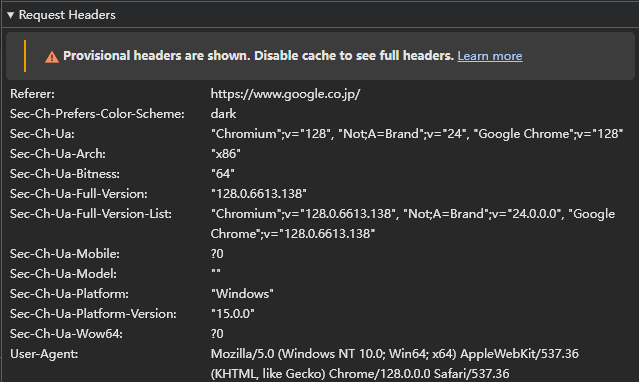
\includegraphics[width=\textwidth]{figures/GET2.png}
    \caption{GET方法对应报文}\label{GET2}
\end{figure}

\subsubsection{POST方法}
图\ref{POST1},\ref{POST2}为\url{google.co.jp}发出的一个POST方式的请求和对应响应的报文内容。

在General菜单中,Request URL字段表明该请求所需资源的URL为\url{https://www.google.co.jp/log?format=json&hasfast=true};
Request Method字段表明该请求的方法为POST;
Status Code字段表明请求成功,状态码为200。

在Response Headers菜单中,
Cache-Control字段表明客户端可以缓存该数据;
Content-Encoding,Content-Length和Content-Type字段分别说明了该数据的编码方式、长度以及类型;
Set-Cookie字段为服务端为客户端设置的Cookie,其中还包含着失效日期Thu,20-Mar-2025 14:19:21 GMT、域名.google.com等信息。

在Request Headers菜单中, 
Referer字段表明该请求从\url{https://www.google.co.jp/}发送;
Accept字段表明客户端接受任何类型的响应(*/*);
path字段中可以获取报文体format=json\&hasfast=true,通知客户端所需格式为json,并且设置hasfast为true,同时还告诉我们该请求的目的是登录。
\begin{figure}[!htbp]
    \centering
    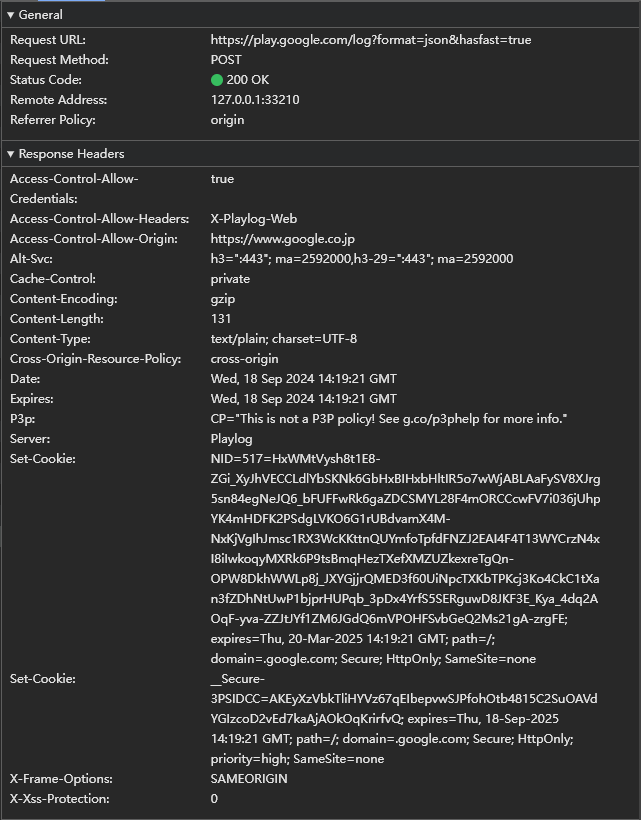
\includegraphics[width=\textwidth]{figures/POST1.png}
    \caption{POST方法对应报文}\label{POST1}
\end{figure}
\begin{figure}[!htbp]
    \centering
    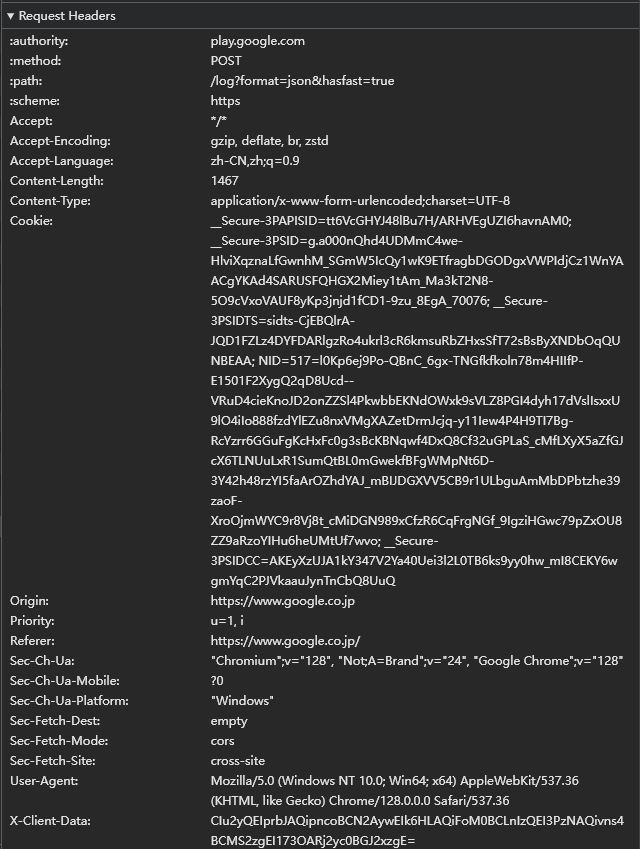
\includegraphics[width=\textwidth]{figures/POST2.png}
    \caption{POST方法对应报文}\label{POST2}
\end{figure}






